\setcounter{secnumdepth}{1}
\section{Einführung}
Diese Bachelorarbeit behandelt die Ausführung und Verarbeitung von asynchronen Prozessen in der Programmierung speziell in der Sprache Typescript.\\
Zielgruppe dieser Arbeit sind Personen, die Grundkenntnisse in der Sprache Javascript/Typescript vorweisen können.
Sollte man von der Skriptsprache Typescript noch nicht/kaum etwas gehört haben, sollte vor dem Lesen dieser Arbeit die Offizielle Dokumentation von Microsoft durchgegangen werden.

\begin{center}
\url{https://www.typescriptlang.org/docs/home.html}
\end{center}

In dieser Arbeit wird nur oberflächlich auf die Unterschiede der beiden Sprachen eingegangen. Des Weiteren sollte man von den Kernkonzepten der Promises und Observables schon mal gehört haben, da diese in der Arbeit gegenübergestellt werden.

\subsection{Typescript}
Typescript. Bereits der Name sagt schon was diese Sprache ausmacht. Sie \textit{(\glqq{}Type\grqq{} zu deutsch: Typ)} ist eine typisierte Form der Skriptsprache Javascript. In Typescript ist es Standard, jede Variable, Funktion und Funktionsparameter im Vorfeld zu typisieren. Mit dem Typescript Compiler werden Dateien mit dem Suffix *.ts in *.js überführt. Zur Laufzeit werden Fehler im Code vom Typescript-Compiler entdeckt.

\subsubsection{Beispiel}

\begin{figure}[h!]
\begin{lstlisting}
class Greeter {
    greeting: string;
    constructor (message: string) {
        this.greeting = message;
    }
    greet() {
        return "Hello, " + this.greeting;
    }
}  
\end{lstlisting}
\caption{Typescript Klasse \cite{typescript-example}}
\end{figure}

Im oberen Code-Schnipsel wurden die variablen und die Klassenmethoden nach Typescript-Standard deklariert. Diese Typen werden beim übersetzen in Javascript ignoriert. Der Kompiler einer Entwicklungsumgebung prüft dann, ob beim übergeben eines Parameters in den Konstruktor ein numerischer oder Boolean-Wert eingesetzt wird. Dies wird dann als ein Fehler erkannt. Der Kompiler übersetzt auch nicht direkt deklarierte Typen. Wie in diesem Fall wird erkannt, dass die Methode greet() einen String-Wert zurückgibt.

\begin{figure}[t]
\begin{lstlisting}
var Greeter = (function () {
    function Greeter(message) {
        this.greeting = message;
    }
    Greeter.prototype.greet = function () {
        return "Hello, " + this.greeting;
    };
    return Greeter;
})(); 
\end{lstlisting}
\caption{Überführung in Javascript \cite{typescript-example}}
\end{figure}
In der vom Kompiler auf Javascript übersetzten Version werden die erstellten Klassen und Typen vollständig eliminiert. Was verbleibt ist die Übersetzung der Klassen-Methode greet() und des Konstruktors in einer Funktion. Sowohl Klassen als auch Interfaces werden in Javascript nicht genutzt.
\\\\
Da Syntaktisch alles was auf Javascript geschrieben auch valider Typescript Code ist, kann man Typescript als Superset von Javascript bezeichnen.
Wichtig zu erwähnen ist, dass diese Sprache optionale statische Typen, Klassen und Interfaces bietet, diese sind jedoch keine Pflicht in der Anwendung. Es ist lediglich eine Konvention.
Nichtsdestotrotz findet Typescript immer mehr Beliebtheit in Unternehmensprojekten. Entwicklerteams können durch die Typisierung schneller Bugs am Code erkennen und durch den modularen Aufbau, den Typescript ermöglicht, die Organisation und Dokumentation von großen Projekten verbessern. Diese Tendenz wird von der beliebten Entwicklerplattform Stackoverflow untermauert, die laut einer Umfrage welche die beliebtesten Programmiersprachen unter Entwickler sei, folgendes rauskam:

\begin{figure}[H]
\centering
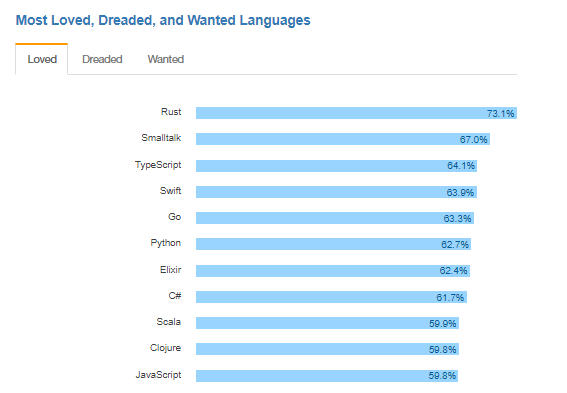
\includegraphics[height=6cm]{stackoverflow-typescript-popularity}
\caption{Prozentualer Anteil der Entwickler die Interesse an neuen Technologien zeigen und weiter mit neuen Technologien arbeiten möchten. \cite{typescript-survey}}
\end{figure}

\subsection{Vorbereitung}
\subsubsection{Tooling}
Um unser Typescript-Beispielprojekt modular zu gestalten, brauchen wir die Hilfe eines sog.\glqq Module-Bundlers\grqq{}. Code-splitting und die Unterteilung in Module wollen wir aus dem Grund der Übersichtlichkeit sowie der einfachen Verwaltung des Codes machen. Es ist eine klassische Programmierpraxis, bekannt aus den Programmiersprachen wie C, C++, PHP, Ruby, Python usw. Das Problem bei kompiliertem Javascript in einem Internetbrowser ist, dass es nativ kein Code-splitting unterstützt. Alle Skripte werden im Rahmen eines Kontexts im Browser bearbeitet, in der Reihenfolge, in der sie aus einem HTML-Format parsiert werden. Und hier kommt Webpack ins Spiel.  \cite{webpack-einfuehrung}
\\\\
Typescript setzt auf Klassen. Heutzutage trennt die Schreibweise in Javascript und Typescript allerdings nur noch die Typisierung, weshalb hier der Mehrwert inzwischen geringer ist. Ansonsten bietet Typescript auch die Möglichkeit zu einem modularen Programmieren, allerdings muss das Verknüpfen zusätzlich von außen durch einen Module-Loader gestemmt werden, Typescript selbst kennt nur Methoden zum Im- und Exportieren.

Um einen modularen Aufbau des Projektes zu gewährleisten, wird das Build-Tool \glqq{}Webpack\grqq{} verwendet. Bei Webpack handelt es sich um einen \glqq{}static module bundler\grqq{} für JavaScript-Anwendungen. Die Idee dahinter ist, einen Dependency-Graphen aufzubauen, der alle JavaScript-Module der Anwendung enthält und diese in ein (oder mehrere) Bundle packt. Zusätzlich können CSS-Module und HMTL-Module gebündelt werden. So kann Code separat abgekapselt werden.\cite{Webpack-basics}

\begin{enumerate} 
\item Motivation hinter der bachelorarbeit
\item Was kann man aus dieser Bachelorarbeit "gewinnen"?
\end{enumerate}

\section{Vorbereitung}
\begin{enumerate} 
\item Welches Framework wird verwendet (Wenn überhaupt?) und welche Sprache angewandt?
\item Repo-Referenz
\end{enumerate}

\subsection{Einführung in asynchrone Operationen}
*Source-code Beispiel*